\tikzset{every picture/.style={line width=0.75pt}} %set default line width to 0.75pt        

\begin{tikzpicture}[x=0.75pt,y=0.75pt,yscale=-1,xscale=1]
\path (0,717);

\path[fill=nodecolor, draw=black, rounded corners=10pt, general shadow={fill={rgb, 255:red, 155; green, 155; blue, 155 },shadow xshift=-3pt,shadow yshift=-3pt}
	] (95,160) rectangle +(985,310) 
	node (logo) [scale=0.4,pos=.09,xshift=1600] {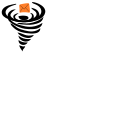
\includegraphics[width=75.75pt,height=90.23pt]{../../../../website/src/main/jbake/assets/images/MessageVortexLogo}}
	node (text) [scale=2.5,pos=.08,xshift=12] {VortexNode};

% Accounting
\draw[fill=layercolor, draw=black,rounded corners=10pt,	general shadow={fill=nodeshadow,shadow xshift=-3pt,shadow yshift=-3pt}
	] (110,230) rectangle +(960,70)  node  [font=\footnotesize, pos=.5, scale=1.8] [align=left] {Accounting};;

% Routing
\draw[fill=layercolor, draw=black,rounded corners=10pt,	general shadow={fill=nodeshadow,shadow xshift=-3pt,shadow yshift=-3pt}
	] (110,310) rectangle +(960,70)  node  [font=\footnotesize, pos=.5, scale=1.8] [align=left] {Routing};;

% Blending
\draw[fill=layercolor, draw=black,rounded corners=10pt,	general shadow={fill=nodeshadow,shadow xshift=-3pt,shadow yshift=-3pt}
	] (110,390) rectangle +(300,70)  node  [font=\footnotesize, pos=.5, scale=1.8] [align=left] {Blending};;
\draw[fill=layercolor, draw=black,rounded corners=10pt,	general shadow={fill=nodeshadow,shadow xshift=-3pt,shadow yshift=-3pt}
	] (440,390) rectangle +(300,70)  node  [font=\footnotesize, pos=.5, scale=1.8] [align=left] {Blending};;
\draw[fill=layercolor, draw=black,rounded corners=10pt,	general shadow={fill=nodeshadow,shadow xshift=-3pt,shadow yshift=-3pt}
	] (770,390) rectangle +(300,70)  node  [font=\footnotesize, pos=.5, scale=1.8] [align=left] {Blending};;


% Transport
\draw[fill=transportcolor, draw=black,rounded corners=10pt,	general shadow={fill=nodeshadow,shadow xshift=-3pt,shadow yshift=-3pt}
	] (110,480) rectangle +(300,70)  node  [font=\footnotesize, pos=.5, scale=1.8] [align=left] {\textcolor{white}{Transport}};;
\draw[fill=transportcolor, draw=black,rounded corners=10pt,	general shadow={fill=nodeshadow,shadow xshift=-3pt,shadow yshift=-3pt}
	] (440,480) rectangle +(300,70)  node  [font=\footnotesize, pos=.5, scale=1.8] [align=left] {\textcolor{white}{Transport}};;
\draw[fill=transportcolor, draw=black,rounded corners=10pt,	general shadow={fill=nodeshadow,shadow xshift=-3pt,shadow yshift=-3pt}
	] (770,480) rectangle +(140,70)  node  [font=\footnotesize, pos=.5, scale=1.7] [align=left] {\textcolor{white}{Transport In}};;
\draw[fill=transportcolor, draw=black,rounded corners=10pt,	general shadow={fill=nodeshadow,shadow xshift=-3pt,shadow yshift=-3pt}
	] (930,480) rectangle +(140,70)  node  [font=\footnotesize, pos=.5, scale=1.7] [align=left] {\textcolor{white}{Transport Out}};;

\end{tikzpicture}